\section{Spektrum Frekuensi Eigen Mode Kuasinormal}
\label{sec:spektrum}

\noindent Bagian ini membahas hasil spektrum frekuensi yang diperoleh pada masing-masing ruang-waktu terhadap variasi parameter geometrinya, yaitu massa lubang hitam ($M$) pada ruang-waktu Schwarzschild dan jari-jari horizon peristiwa ($r_+$) pada ruang-waktu Schwarzschild Anti-de Sitter. Pada masing-masing ruang-waktu, spektrum frekuensi turut dianalisis terhadap variasi momentum sudut ($\ell = 0, 1, 2$), dengan fokus pada mode fundamental ($n=0$) dan overtone pertama ($n=1$).

\subsection{Schwarzschild}
\label{subsec:frek-sch}

Pembahasan diawali dengan analisis spektrum frekuensi mode kuasinormal pada ruang-waktu Schwarzschild. Variasi massa lubang hitam yang digunakan dalam penelitian ini berada pada rentang $M = 0.2,\;0.33,\;0.47,\;0.60,\;0.73,\;0.87,\;\text{dan}\;1.0$, yang dipilih untuk mengamati perubahan spektrum frekuensi kuasinormal terhadap peningkatan massa lubang hitam. Pada setiap kombinasi momentum sudut dan indeks overtone, analisis dilakukan untuk dua kondisi medan skalar, yaitu medan tak bermassa ($\mu=0$) dan medan bermassa ($\mu=1$), sehingga pengaruh massa medan terhadap spektrum frekuensi dapat diamati secara sistematis.

\subsubsection*{Medan Skalar Tak Bermassa ($\mu=0$)}

\begin{table}[H]
\centering
\caption{Spektrum frekuensi mode kuasinormal medan skalar tak bermassa ($\mu=0$) pada ruang-waktu Schwarzschild untuk mode fundamental ($n=0$).}
\vspace{0.2cm}
\renewcommand{\arraystretch}{1.25}
\begin{tabular}{cccc}
\toprule
$M$ & $\omega(\ell=0)$ & $\omega(\ell=1)$ & $\omega(\ell=2)$ \\
\midrule
0.20 & $0.5525 - 0.5245i$ & $1.4645 - 0.4885i$ & $2.4180 - 0.4840i$ \\
0.33   & $0.3315 - 0.3147i$ & $0.8787 - 0.2931i$ & $1.4508 - 0.2904i$ \\
0.47   & $0.2368 - 0.2248i$ & $0.6276 - 0.2094i$ & $1.0363 - 0.2074i$ \\
0.60   & $0.1842 - 0.1748i$ & $0.4882 - 0.1628i$ & $0.8060 - 0.1613i$ \\
0.73   & $0.1507 - 0.1430i$ & $0.3994 - 0.1332i$ & $0.6595 - 0.1320i$ \\
0.87   & $0.1275 - 0.1210i$ & $0.3380 - 0.1127i$ & $0.5580 - 0.1117i$ \\
1.00    & $0.1105 - 0.1049i$ & $0.2929 - 0.0977i$ & $0.4836 - 0.0968i$ \\
\bottomrule
\end{tabular}
\label{tab:sch_mu0_n0}
\end{table}

Tabel \ref{tab:sch_mu0_n0} menunjukkan spektrum frekuensi mode kuasinormal medan skalar tak bermassa ($\mu=0$) pada berbagai variasi massa lubang hitam untuk mode fundamental ($n=0$). Terlihat bahwa peningkatan massa lubang hitam menyebabkan baik bagian real ($\omega_R$) maupun bagian imajiner ($\omega_I$) mengalami penurunan untuk seluruh nilai momentum sudut yang ditinjau. Sebagai contoh, pada mode $\ell=0$, bagian real menurun dari $0.5525$ ($M=0.2$) menjadi $0.1105$ ($M=1.0$), sedangkan bagian imajiner menurun dari $0.5245$ menjadi $0.1049$. Hasil yang serupa juga terlihat pada nilai parameter sudut yang berbeda, $\ell=1$ dan $\ell=2$. Momentum sudut memberikan pengaruh yang signifikan terhadap bagian frekuensi real, yakni pada $M=1.0$, nilai $\omega_R$ mengalami peningkatan yang cukup jelas dari $0.1105$ menjadi $0.2929$ dan $0.4836$ untuk $\ell=0$, $\ell=1$, dan $\ell=2$, sedangkan perubahan pada bagian imajiner relatif lebih kecil.

\begin{table}[H]
\centering
\caption{Spektrum frekuensi mode kuasinormal medan skalar tak bermassa ($\mu=0$) pada ruang-waktu Schwarzschild untuk overtone pertama ($n=1$).}
\vspace{0.2cm}
\renewcommand{\arraystretch}{1.25}
\begin{tabular}{cccc}
\toprule
$M$ & $\omega(\ell=0)$ & $\omega(\ell=1)$ & $\omega(\ell=2)$ \\
\midrule
0.20 & $0.4305 - 1.7405i$ & $1.3225 - 1.5315i$ & $2.3195 - 1.4780i$ \\
0.33   & $0.2583 - 1.0443i$ & $0.7935 - 0.9189i$ & $1.3917 - 0.8868i$ \\
0.47   & $0.1845 - 0.7459i$ & $0.5668 - 0.6564i$ & $0.9941 - 0.6334i$ \\
0.60   & $0.1435 - 0.5802i$ & $0.4408 - 0.5105i$ & $0.7732 - 0.4927i$ \\
0.73   & $0.1174 - 0.4747i$ & $0.3607 - 0.4177i$ & $0.6326 - 0.4031i$ \\
0.87   & $0.0993 - 0.4017i$ & $0.3052 - 0.3534i$ & $0.5353 - 0.3411i$ \\
1.00    & $0.0861 - 0.3481i$ & $0.2645 - 0.3063i$ & $0.4639 - 0.2956i$ \\
\bottomrule
\end{tabular}
\label{tab:sch_mu0_n1}
\end{table}

Tabel~\ref{tab:sch_mu0_n1} menunjukkan spektrum frekuensi mode kuasinormal medan skalar tak bermassa ($\mu=0$) untuk overtone pertama ($n=1$), dengan variasi massa lubang hitam dan momentum sudut yang sama seperti pada mode fundamental. Peningkatan massa lubang hitam kembali menyebabkan penurunan baik pada bagian real ($\omega_R$) maupun bagian imajiner ($\omega_I$) untuk seluruh nilai momentum sudut yang ditinjau. Kecenderungan tersebut serupa dengan yang diperoleh pada mode fundamental, yaitu semakin besar massa lubang hitam maka frekuensi osilasi maupun laju peluruhan perturbasi menjadi semakin kecil. Hal ini menunjukkan bahwa pengaruh massa lubang hitam terhadap spektrum frekuensi kuasinormal tetap dipertahankan ketika indeks \textit{overtone} dinaikkan menjadi $n=1$.

Dibandingkan dengan mode fundamental, \textit{overtone} pertama menunjukkan karakteristik spektrum yang berbeda. Secara umum, bagian real frekuensi cenderung lebih kecil, sedangkan bagian imajiner frekuensi lebih besar dibandingkan mode fundamental untuk setiap peningkatan massa lubang hitam dan momentum sudut yang sama. Dengan demikian, mode \textit{overtone} pertama berosilasi pada frekuensi yang lebih rendah, namun mengalami peluruhan yang lebih cepat daripada mode fundamental.

%%%%%%%%%%%%%%%%%%%%%%%%%%%%%%%%%%%%%%%%%%%%%%%%%%%%%%%%%%%%%%%%%%%%%%
%% MASSIVE FUNDAMENTAL
%%%%%%%%%%%%%%%%%%%%%%%%%%%%%%%%%%%%%%%%%%%%%%%%%%%%%%%%%%%%%%%%%%%%%%

\subsubsection*{Medan Skalar Bermassa ($\mu=1$)}

Bagian ini membahas spektrum frekuensi untuk medan skalar bermassa dengan menetapkan massa medan sebesar $\mu=1$. Analisis dimulai dari mode fundamental ($n=0$), kemudian dilanjutkan dengan \textit{overtone} pertama ($n=1$) untuk mengamati kecenderungan yang diperoleh pada mode fundamental pada \textit{overtone} yang lebih tinggi.

\begin{table}[H]
\centering
\caption{Spektrum frekuensi mode kuasinormal medan skalar bermassa ($\mu=1$) pada ruang-waktu Schwarzschild untuk mode fundamental ($n=0$)}
\vspace{0.2cm}
\renewcommand{\arraystretch}{1.25}
\begin{tabular}{cccc}
\toprule
$M$ & $\omega(\ell=0)$ & $\omega(\ell=1)$ & $\omega(\ell=2)$ \\
\midrule
0.20 & $0.5810 - 0.3768i$ & $1.5548 - 0.4330i$ & $2.4816 - 0.4619i$ \\
0.33 & $0.3739 - 0.0967i$ & $1.0303 - 0.1948i$ & $1.5575 - 0.2532i$ \\
0.47 & $0.2877 - 0.0157i$ & $0.8378 - 0.0578i$ & $1.1875 - 0.1536i$ \\
0.60 & - & - & $1.0038 - 0.0881i$ \\
0.73 & - & - & $0.9052 - 0.0341i$ \\
0.87 & - & - & - \\
1.00 & - & - & - \\
\bottomrule
\end{tabular}
\label{tab:sch_mu1_n0}
\end{table}

Tabel~\ref{tab:sch_mu1_n0} menyajikan spektrum frekuensi mode kuasinormal medan skalar bermassa ($\mu=1$) untuk mode fundamental ($n=0$). Penambahan massa medan skalar menyebabkan perubahan yang cukup signifikan pada spektrum frekuensi mode kuasinormal untuk seluruh nilai massa lubang hitam dan momentum sudut yang ditinjau. Meninjau dengan hasil pada Tabel~\ref{tab:sch_mu0_n0}, bagian real frekuensi ($\omega_R$) tetap mengalami penurunan seiring bertambahnya massa lubang hitam, dan bagian imajiner ($\omega_I$) juga menunjukkan kecenderungan menurun hingga akhirnya metode numerik tidak lagi berhasil menemukan akar yang konvergen pada beberapa variasi nilai massa lubang hitam yang lebih besar. Perubahan tersebut menunjukkan bahwa ditambahkannya massa medan sangat memengaruhi kedua bagian frekuensi.

Selain itu, pengaruh momentum sudut pada mode fundamental menunjukkan kecenderungan yang
serupa dengan kasus tak bermassa. Untuk setiap variasi massa lubang hitam, peningkatan
momentum sudut dari $\ell=0$ hingga $\ell=2$ menyebabkan baik bagian real maupun bagian
imajiner frekuensi meningkat. Hal ini menunjukkan bahwa momentum sudut tetap memperbesar frekuensi osilasi
sekaligus laju peluruhan perturbasi ketika medan skalar diberi massa.
%%%%%%%%%%%%%%%%%%%%%%%%%%%%%%%%%%%%%%%%%%%%%%%%%%%%%%%%%%%%%%%%%%%%%%
%% MASSIVE OVERTONE
%%%%%%%%%%%%%%%%%%%%%%%%%%%%%%%%%%%%%%%%%%%%%%%%%%%%%%%%%%%%%%%%%%%%%%

\begin{table}[H]
\centering
\caption{Spektrum frekuensi mode kuasinormal medan skalar bermassa ($\mu=1$) pada ruang-waktu Schwarzschild untuk overtone pertama ($n=1$).}
\vspace{0.2cm}
\renewcommand{\arraystretch}{1.25}
\begin{tabular}{cccc}
\toprule
$M$ & $\omega(\ell=0)$ & $\omega(\ell=1)$ & $\omega(\ell=2)$ \\
\midrule
0.20 & $0.4097 - 1.7136i$ & $1.3256 - 1.4639i$ & $2.3514 - 1.4309i$ \\
0.33 & $0.2326 - 0.9980i$ & $0.7940 - 0.8105i$ & $1.4442 - 0.8070i$ \\
0.47 & $0.1595 - 0.6774i$ & $0.5623 - 0.5149i$ & $1.0652 - 0.5191i$ \\
0.60 & $0.1219 - 0.4873i$ & $0.4337 - 0.3428i$ & $0.8590 - 0.3423i$ \\
0.73 & $0.1001 - 0.3566i$ & $0.3544 - 0.2267i$ & $0.7280 - 0.2175i$ \\
0.87 & $0.0862 - 0.2591i$ & $0.3019 - 0.1399i$ & $0.6368 - 0.1236i$ \\
1.00 & $0.0728 - 0.1822i$ & $0.2632 - 0.0709i$ & $0.5704 - 0.0492i$ \\
\bottomrule
\end{tabular}
\label{tab:sch_mu1_n1}
\end{table}

Tabel~\ref{tab:sch_mu1_n1} menunjukkan spektrum frekuensi mode kuasinormal medan skalar bermassa ($\mu=1$) untuk overtone pertama ($n=1$). Nilai frekuensi kuasinormal pada \textit{overtone} pertama masih menunjukkan ketergantungan yang jelas terhadap massa lubang hitam maupun momentum sudut. Seiring meningkatnya massa lubang hitam, bagian real frekuensi ($\omega_R$) maupun bagian imajiner ($\omega_I$) sama-sama mengalami penurunan untuk seluruh nilai momentum sudut yang ditinjau. Namun, dibandingkan dengan mode fundamental pada Tabel~\ref{tab:sch_mu1_n0}, peningkatan indeks \textit{overtone} menghasilkan pengaruh yang berbeda pada kedua komponen frekuensi: bagian real cenderung menurun, sedangkan bagian imajiner justru meningkat cukup signifikan. Hal ini menunjukkan bahwa mode \textit{overtone} pertama berosilasi pada frekuensi yang lebih rendah, namun mengalami peluruhan yang jauh lebih cepat dibandingkan mode fundamental.

%%%%%%%%%%%%%%%%%%%%%%%%%%%%%%%%%%%%%%%%%%%%%%%%%%%%%%%%%%%%%%%%%%%%%%
%% GRAFIK SAF
%%%%%%%%%%%%%%%%%%%%%%%%%%%%%%%%%%%%%%%%%%%%%%%%%%%%%%%%%%%%%%%%%%%%%%

Guna mempermudah perbandingan keempat hasil spektrum frekuensi yang telah dipaparkan, data pada keempat tabel tersebut divisualisasikan dalam bentuk grafik perbandingan antara bagian real ($\omega_R$) dan bagian imajiner ($\omega_I$) terhadap massa lubang hitam ($M$), sebagaimana ditunjukkan pada Gambar~\ref{fig:saf_n0} untuk mode fundamental dan Gambar~\ref{fig:saf_n1} untuk overtone pertama.

\begin{figure}[H]
\centering

\begin{subfigure}[t]{0.48\textwidth}
\centering
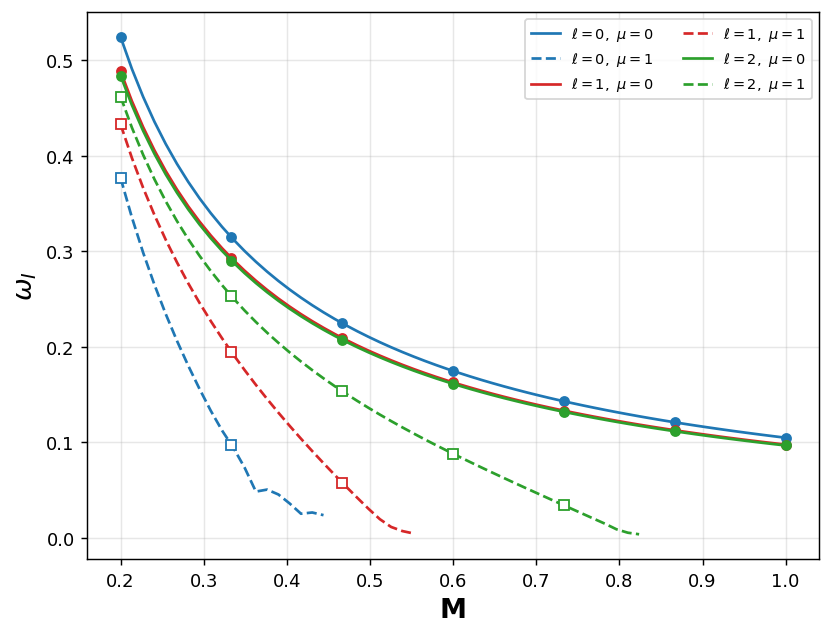
\includegraphics[width=\linewidth]{uploads/Gambar Hasil/grafik_saf_overtone_n0_imajiner.png}
\caption{$\omega_I$ terhadap massa lubang hitam.}
\label{fig:saf_n0_wI}
\end{subfigure}
\hfill
\begin{subfigure}[t]{0.48\textwidth}
\centering
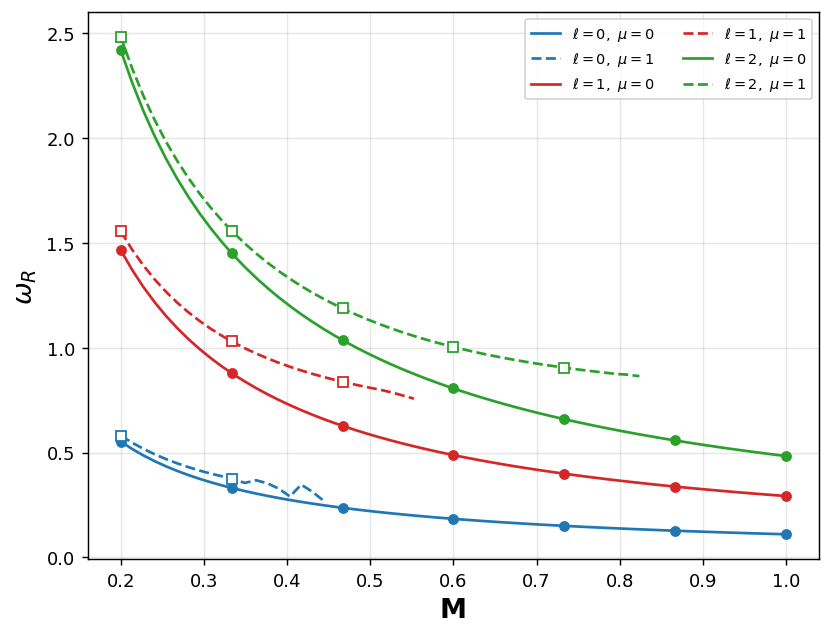
\includegraphics[width=\linewidth]{uploads/Gambar Hasil/grafik_saf_overtone_n0_riil.png}
\caption{$\omega_R$ terhadap massa lubang hitam.}
\label{fig:saf_n0_wR}
\end{subfigure}

\caption{
Perbandingan spektrum frekuensi mode kuasinormal medan skalar pada ruang-waktu Schwarzschild terhadap massa lubang hitam ($M$) untuk mode fundamental ($n=0$). Garis penuh menyatakan medan skalar tak bermassa ($\mu=0$), sedangkan garis putus-putus menyatakan medan skalar bermassa ($\mu=1$). Kurva berwarna biru, merah, dan hijau masing-masing merepresentasikan momentum sudut $\ell=0$, $\ell=1$, dan $\ell=2$.
}
\label{fig:saf_n0}

\end{figure}

Gambar~\ref{fig:saf_n0} memvisualisasikan tren pada Tabel~\ref{tab:sch_mu0_n0} dan Tabel~\ref{tab:sch_mu1_n0} secara bersamaan. Seluruh kurva $\omega_I$ dan $\omega_R$ terlihat menurun secara monotonik seiring bertambahnya $M$, sementara kurva medan bermassa ($\mu=1$, garis putus-putus) tampak terputus lebih awal dibandingkan kurva medan tak bermassa, mengonfirmasi secara visual batas konvergensi numerik yang telah disebutkan sebelumnya.

\begin{figure}[H]
\centering

\begin{subfigure}[t]{0.48\textwidth}
\centering
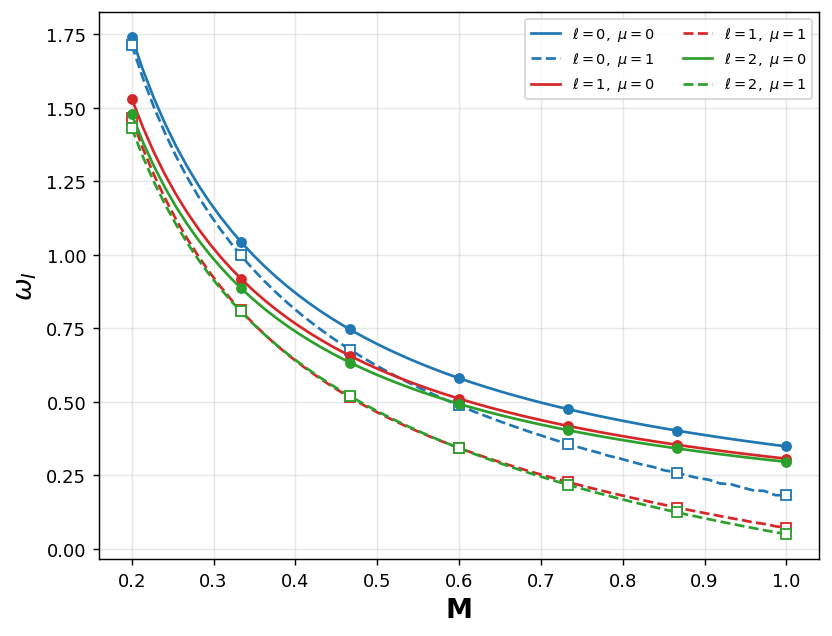
\includegraphics[width=\linewidth]{uploads/Gambar Hasil/grafik_saf_overtone_n1_imajiner.png}
\caption{$\omega_I$ terhadap massa lubang hitam.}
\label{fig:saf_n1_wI}
\end{subfigure}
\hfill
\begin{subfigure}[t]{0.48\textwidth}
\centering
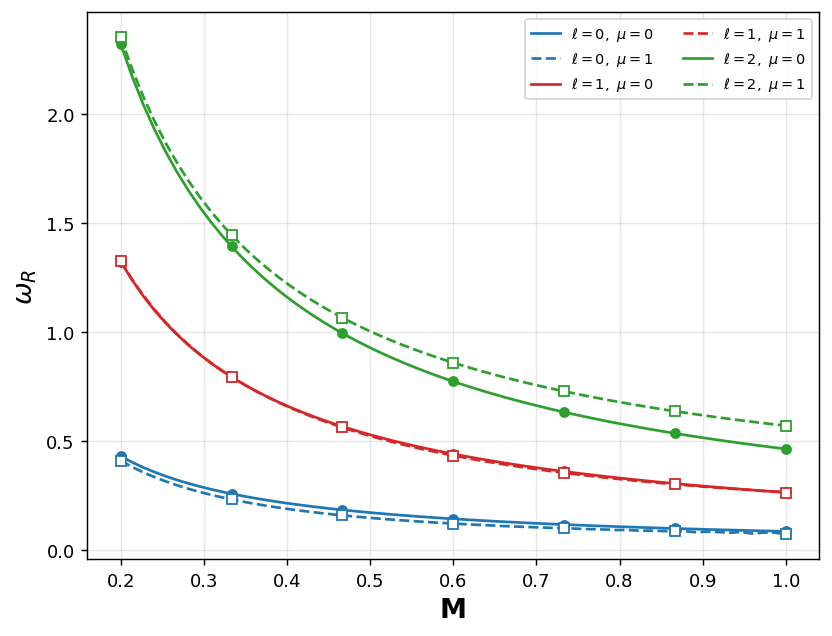
\includegraphics[width=\linewidth]{uploads/Gambar Hasil/grafik_saf_overtone_n1_riil.png}
\caption{$\omega_R$ terhadap massa lubang hitam.}
\label{fig:saf_n1_wR}
\end{subfigure}

\caption{
Perbandingan spektrum frekuensi mode kuasinormal medan skalar pada ruang-waktu Schwarzschild terhadap massa lubang hitam ($M$) untuk overtone pertama ($n=1$). Garis penuh menyatakan medan skalar tak bermassa ($\mu=0$), sedangkan garis putus-putus menyatakan medan skalar bermassa ($\mu=1$). Kurva berwarna biru, merah, dan hijau masing-masing merepresentasikan momentum sudut $\ell=0$, $\ell=1$, dan $\ell=2$.
}
\label{fig:saf_n1}

\end{figure}

Pola serupa juga teramati pada Gambar~\ref{fig:saf_n1} untuk overtone pertama, dengan kurva $\omega_I$ berada pada rentang nilai yang lebih tinggi dibandingkan Gambar~\ref{fig:saf_n0}, sejalan dengan laju peluruhan overtone yang lebih cepat daripada mode fundamental. Keterputusan dini kurva medan bermassa juga masih tampak, khususnya pada momentum sudut yang lebih kecil.

\subsection{Schwarzschild Anti-de Sitter}
\label{subsec:frek-sads}

Setelah membahas spektrum frekuensi pada ruang-waktu Schwarzschild, analisis selanjutnya dilakukan pada ruang-waktu Schwarzschild Anti-de Sitter (SAdS). Berbeda dengan kasus Schwarzschild yang dikarakterisasi oleh perubahan nilai massa lubang hitam ($M$), karakteristik geometri SAdS ditentukan oleh perubahan jari-jari horizon peristiwa yang relatif terhadap suatu nilai acuan horizon peristiwa ($r_+$), dengan variasi $r_+=0.4,\;0.8,\;1.0,\;5.0,\;10.0,\;50.0,\;\text{dan}\;100.0$ yang dipilih untuk mengamati perubahan spektrum frekuensi kuasinormal terhadap peningkatan ukuran horizon peristiwa. Pada setiap kombinasi momentum sudut dan indeks overtone, analisis dilakukan untuk dua kondisi medan skalar, yaitu medan tak bermassa ($\mu=0$) dan medan bermassa ($\mu=1$), sehingga pengaruh massa medan terhadap spektrum frekuensi dapat diamati secara sistematis.

\subsubsection*{Medan Skalar Tak Bermassa ($\mu=0$)}

\begin{table}[H]
\centering
\caption{Spektrum frekuensi mode kuasinormal medan skalar tak bermassa ($\mu=0$) pada ruang-waktu Schwarzschild Anti-de Sitter untuk mode fundamental ($n=0$).}
\vspace{0.2cm}
\renewcommand{\arraystretch}{1.25}
\begin{tabular}{cccc}
\toprule
$r_+$ & $\omega(\ell=0)$ & $\omega(\ell=1)$ & $\omega(\ell=2)$ \\
\midrule
0.4   & $2.3629 - 1.0065i$ & $3.1338 - 0.7029i$ & $4.1285 - 0.4512i$ \\
0.8   & $2.5878 - 2.1304i$ & $3.1751 - 1.9193i$ & $4.0082 - 1.6917i$ \\
1.0   & $2.7982 - 2.6712i$ & $3.3306 - 2.4895i$ & $4.1171 - 2.2756i$ \\
5.0   & $9.4711 - 13.3255i$ & $9.6323 - 13.2795i$ & $9.9426 - 13.1924i$ \\
10.0  & $18.6070 - 26.6418i$ & $18.6895 - 26.6185i$ & $18.8527 - 26.5725i$ \\
50.0  & $92.4937 - 133.1933i$ & $92.5103 - 133.1886i$ & $92.5435 - 133.1792i$ \\
100.0 & $184.9534 - 266.3856i$ & $184.9618 - 266.3833i$ & $184.9784 - 266.3786i$ \\
\bottomrule
\end{tabular}
\label{tab:sads_mu0_n0}
\end{table}

Tabel \ref{tab:sads_mu0_n0} menunjukkan spektrum frekuensi mode kuasinormal medan skalar tak bermassa ($\mu=0$) untuk mode fundamental ($n=0$) pada variasi jari-jari horizon peristiwa yang dipilih. Terlihat bahwa jari-jari horizon peristiwa memberikan pengaruh yang signifikan terhadap spektrum frekuensi mode kuasinormal pada ruang-waktu Schwarzschild Anti-de Sitter. Seiring bertambahnya nilai $r_+$, baik bagian real ($\omega_R$) maupun bagian imajiner ($\omega_I$) menunjukkan kecenderungan meningkat untuk seluruh nilai momentum sudut yang ditinjau. Sebagai contoh, pada mode $\ell=0$, bagian real meningkat dari $2.3629$ ($r_+=0.4$) menjadi $184.9534$ ($r_+=100.0$), sedangkan bagian imajiner meningkat dari $1.0065$ ($r_+ = 0.4$) menjadi $266.3856$ ($r_+ = 100.0$). Kecenderungan ini berbanding terbalik dengan perilaku pada lubang hitam Schwarzschild, sehingga mengindikasikan bahwa peningkatan ukuran horizon peristiwa pada SAdS justru meningkatkan frekuensi osilasi maupun laju peluruhan perturbasi medan skalar.

Pengaruh momentum sudut pada Schwarzschild Anti-de Sitter berkebalikan dengan pengaruhnya pada ruang-waktu Schwarzschild. Pada Schwarzschild, nilai kedua bagian frekuensi mengalami kenaikan seiring meningkatnya nilai parameter momentum sudut, namun pada Schwarzschild Anti-de Sitter menurunkan nilai laju peluruhannya. Hal ini kemudian diinterpretasikan bahwa pada SAdS frekuensi osilasi lubang hitam akan meningkat, namun laju kestabilan lubang hitam akan lebih lama seiring meningkatnya nilai momentum sudut.
%%%%%%%%%%%%%%%%%%%%%%%%%%%%%%%%%%%%%%%%%%%%%%%%%%%%%%%%%%%%%%%%%%%%%%
%% MASSLESS OVERTONE
%%%%%%%%%%%%%%%%%%%%%%%%%%%%%%%%%%%%%%%%%%%%%%%%%%%%%%%%%%%%%%%%%%%%%%

\begin{table}[H]
\centering
\caption{Spektrum frekuensi mode kuasinormal medan skalar tak bermassa ($\mu=0$) pada ruang-waktu Schwarzschild Anti-de Sitter untuk overtone pertama ($n=1$).}
\vspace{0.2cm}
\renewcommand{\arraystretch}{1.25}
\begin{tabular}{cccc}
\toprule
$r_+$ & $\omega(\ell=0)$ & $\omega(\ell=1)$ & $\omega(\ell=2)$ \\
\midrule
0.4   & $3.9786 - 2.0728i$ & $4.5679 - 1.7813i$ & $5.3977 - 1.4465i$ \\
0.8   & $4.3950 - 4.0624i$ & $4.8516 - 3.8831i$ & $5.5393 - 3.6357i$ \\
1.0   & $4.7585 - 5.0376i$ & $5.1724 - 4.8881i$ & $5.8165 - 4.6678i$ \\
5.0   & $16.1820 - 24.6164i$ & $16.3049 - 24.5832i$ & $16.5434 - 24.5184i$ \\
10.0  & $31.8017 - 49.1816i$ & $31.8644 - 49.1649i$ & $31.9889 - 49.1317i$ \\
50.0  & $158.1008 - 245.8244i$ & $158.1134 - 245.8210i$ & $158.1387 - 245.8144i$ \\
100.0 & $316.1447 - 491.6435i$ & $316.1510 - 491.6419i$ & $316.1636 - 491.6385i$ \\
\bottomrule
\end{tabular}
\label{tab:sads_mu0_n1}
\end{table}

Hal yang sama terjadi pada \textit{overtone} pertama ($n=1$), sebagaimana ditunjukkan pada Tabel~\ref{tab:sads_mu0_n1}. Peningkatan jari-jari horizon peristiwa kembali memberikan pengaruh yang signifikan terhadap spektrum frekuensi mode kuasinormal pada ruang-waktu Schwarzschild Anti-de Sitter. Sebagaimana pada mode fundamental, baik bagian real ($\omega_R$) maupun bagian imajiner ($\omega_I$) menunjukkan kecenderungan meningkat seiring bertambahnya nilai radius horizon $r_+$. Hal ini menunjukkan bahwa pengaruh ukuran horizon peristiwa terhadap karakteristik spektrum frekuensi masih sama ketika indeks \textit{overtone} dinaikkan.

Jika dibandingkan dengan mode fundamental pada Tabel \ref{tab:sads_mu0_n0}, \textit{overtone} memperlihatkan karakteristik spektrum yang berbeda. Bagian real frekuensi maupun imajiner mengalami peningkatan dibandingkan mode fundamental. Sebagai contoh, pada $\ell=0$ dan $r_+=0.4$, bagian real meningkat dari $2.3629$ (mode fundamental) menjadi $3.9786$ (\textit{overtone}), dan pada bagian imajiner meningkat dari $1.0065$ menjadi $2.0728$.

Pengaruh momentum sudut pada \textit{overtone} menunjukkan kecenderungan yang serupa, yakni frekuensi osilasi akan mengalami peningkatan dan laju peluruhan akan mengalami penurunan.

%%%%%%%%%%%%%%%%%%%%%%%%%%%%%%%%%%%%%%%%%%%%%%%%%%%%%%%%%%%%%%%%%%%%%%
%% MASSIVE FUNDAMENTAL
%%%%%%%%%%%%%%%%%%%%%%%%%%%%%%%%%%%%%%%%%%%%%%%%%%%%%%%%%%%%%%%%%%%%%%

\subsubsection*{Medan Skalar Bermassa ($\mu=1$)}

Bagian ini membahas spektrum frekuensi untuk medan skalar bermassa dengan menetapkan massa medan sebesar $\mu=1$ pada ruang-waktu Schwarzschild Anti-de Sitter. Analisis dimulai dari mode fundamental ($n=0$), kemudian dilanjutkan dengan \textit{overtone} ($n=1$), untuk mengamati kecenderungan frekuensi yang diperoleh.

\begin{table}[H]
\centering
\caption{Spektrum frekuensi mode kuasinormal medan skalar bermassa ($\mu=1$) pada ruang-waktu Schwarzschild Anti-de Sitter untuk mode fundamental ($n=0$).}
\vspace{0.2cm}
\renewcommand{\arraystretch}{1.25}
\begin{tabular}{cccc}
\toprule
$r_+$ & $\omega(\ell=0)$ & $\omega(\ell=1)$ & $\omega(\ell=2)$ \\
\midrule
0.4   & $2.5879 - 1.1654i$ & $3.3288 - 0.8391i$ & $4.3085 - 0.5592i$ \\
0.8   & $2.8417 - 2.4291i$ & $3.3983 - 2.2053i$ & $4.2075 - 1.9579i$ \\
1.0   & $3.0749 - 3.0382i$ & $3.5775 - 2.8460i$ & $4.3376 - 2.6145i$ \\
5.0   & $10.4349 - 15.0814i$ & $10.5843 - 15.0331i$ & $10.8735 - 14.9415i$ \\
10.0  & $20.5037 - 30.1470i$ & $20.5801 - 30.1225i$ & $20.7315 - 30.0743i$ \\
50.0  & $101.9276 - 150.7088i$ & $101.9430 - 150.7039i$ & $101.9737 - 150.6940i$ \\
100.0 & $203.8182 - 301.4159i$ & $203.8259 - 301.4134i$ & $203.8413 - 301.4085i$ \\
\bottomrule
\end{tabular}
\label{tab:sads_mu1_n0}
\end{table}

Tabel~\ref{tab:sads_mu1_n0} menyajikan spektrum frekuensi mode kuasinormal medan skalar bermassa ($\mu=1$) untuk mode fundamental ($n=0$). Penambahan massa medan skalar tidak mengubah kecenderungan spektrum frekuensi mode kuasinormal terhadap ukuran horizon peristiwa pada ruang-waktu Schwarzschild Anti-de Sitter. Seiring bertambahnya jari-jari horizon peristiwa, baik bagian real ($\omega_R$) maupun magnitudo bagian imajiner ($\omega_I$) tetap mengalami peningkatan untuk seluruh nilai momentum sudut yang ditinjau. Meskipun kecenderungannya sama dengan kasus medan skalar tak bermassa, nilai kedua komponen frekuensi pada medan bermassa lebih besar. Dengan demikian, massa medan skalar menggeser spektrum frekuensi ke nilai yang lebih tinggi tanpa mengubah pola ketergantungannya terhadap $r_+$.

Secara kuantitatif, dibandingkan dengan hasil medan skalar tak bermassa pada Tabel \ref{tab:sads_mu0_n0}, penambahan massa medan skalar menghasilkan peningkatan $\omega_R$ yang relatif konsisten untuk seluruh variasi jari-jari horizon peristiwa yang ditinjau. Hal tersebut menunjukkan bahwa pengaruh massa medan terhadap bagian real frekuensi tidak terbatas pada horizon peristiwa berukuran kecil ataupun besar. Pengaruh momentum sudut juga mempertahankan kecenderungan yang sama seperti pada medan skalar tak bermassa, yaitu peningkatan $\ell$ menyebabkan $\omega_R$ meningkat, sedangkan magnitudo $\omega_I$ menurun. Namun, pengaruh momentum sudut tersebut semakin kecil seiring bertambahnya ukuran horizon peristiwa.

Jika dibandingkan dengan ruang-waktu Schwarzschild, penambahan massa medan skalar memberikan pengaruh yang berbeda terhadap bagian imajiner frekuensi. Pada kedua ruang-waktu, massa medan meningkatkan bagian real frekuensi sehingga frekuensi osilasi menjadi lebih besar. Akan tetapi, pada Schwarzschild, penambahan massa medan cenderung menurunkan magnitudo bagian imajiner sehingga peluruhan perturbasi berlangsung lebih lambat, sedangkan pada Schwarzschild Anti-de Sitter, magnitudo bagian imajiner justru meningkat sehingga peluruhan perturbasi berlangsung lebih cepat. Perbedaan ini menunjukkan bahwa respons spektrum frekuensi mode kuasinormal terhadap massa medan dipengaruhi oleh karakteristik geometri ruang-waktu.

%%%%%%%%%%%%%%%%%%%%%%%%%%%%%%%%%%%%%%%%%%%%%%%%%%%%%%%%%%%%%%%%%%%%%%
%% MASSIVE OVERTONE
%%%%%%%%%%%%%%%%%%%%%%%%%%%%%%%%%%%%%%%%%%%%%%%%%%%%%%%%%%%%%%%%%%%%%%

\begin{table}[H]
\centering
\caption{Spektrum frekuensi mode kuasinormal medan skalar bermassa ($\mu=1$) pada ruang-waktu Schwarzschild Anti-de Sitter untuk overtone pertama ($n=1$).}
\vspace{0.2cm}
\renewcommand{\arraystretch}{1.25}
\begin{tabular}{cccc}
\toprule
$r_+$ & $\omega(\ell=0)$ & $\omega(\ell=1)$ & $\omega(\ell=2)$ \\
\midrule
0.4   & $4.2199 - 2.2295i$ & $4.7921 - 1.9340i$ & $5.6061 - 1.5898i$ \\
0.8   & $4.6615 - 4.3539i$ & $5.1026 - 4.1726i$ & $5.7731 - 3.9199i$ \\
1.0   & $5.0473 - 5.3959i$ & $5.4465 - 5.2448i$ & $6.0732 - 5.0205i$ \\
5.0   & $17.1693 - 26.3344i$ & $17.2871 - 26.3010i$ & $17.5161 - 26.2356i$ \\
10.0  & $33.7427 - 52.6115i$ & $33.8028 - 52.5947i$ & $33.9222 - 52.5613i$ \\
50.0  & $167.7517 - 262.9641i$ & $167.7638 - 262.9607i$ & $167.7880 - 262.9540i$ \\
100.0 & $335.4431 - 525.9222i$ & $335.4492 - 525.9206i$ & $335.4613 - 525.9172i$ \\
\bottomrule
\end{tabular}
\label{tab:sads_mu1_n1}
\end{table}

Tabel~\ref{tab:sads_mu1_n1} menunjukkan spektrum frekuensi mode kuasinormal medan skalar bermassa ($\mu=1$) untuk overtone pertama ($n=1$). Spektrum frekuensi tersebut tetap dipengaruhi oleh ukuran horizon peristiwa: seiring bertambahnya nilai $r_+$, baik bagian real ($\omega_R$) maupun bagian imajiner ($\omega_I$) menunjukkan kecenderungan meningkat untuk seluruh nilai momentum sudut yang ditinjau. Hasil tersebut menunjukkan bahwa pengaruh ukuran horizon peristiwa terhadap karakteristik spektrum frekuensi tetap sama ketika medan skalar bermassa dan indeks \textit{overtone} dinaikkan.

Jika dibandingkan dengan mode fundamental pada Tabel~\ref{tab:sads_mu1_n0}, \textit{overtone} pertama menunjukkan peningkatan pada kedua bagian frekuensi. Sebagai contoh, pada $\ell=0$ dan $r_+=0.4$, bagian real meningkat dari $2.5879$ menjadi $4.2199$, sedangkan bagian imajiner meningkat dari $1.1654$ menjadi $2.2295$. Hasil ini menunjukkan bahwa kenaikan indeks \textit{overtone} tidak hanya memengaruhi frekuensi osilasi, tetapi juga laju peluruhan perturbasi medan skalar.

\begin{figure}[H]
\centering

\begin{subfigure}[t]{0.48\textwidth}
\centering
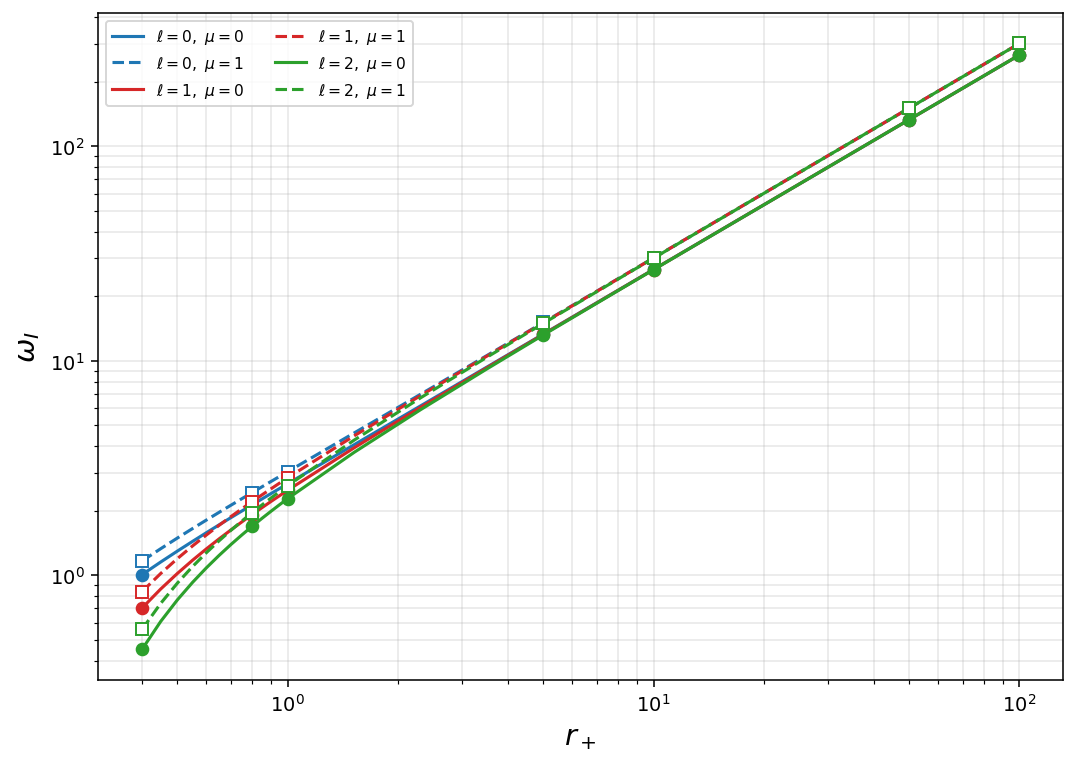
\includegraphics[width=\linewidth]{uploads/Gambar Hasil/grafik_sads_n0_wI.png}
\caption{$\omega_I$ terhadap jari-jari horizon peristiwa.}
\label{fig:sads_n0_wI}
\end{subfigure}
\hfill
\begin{subfigure}[t]{0.48\textwidth}
\centering
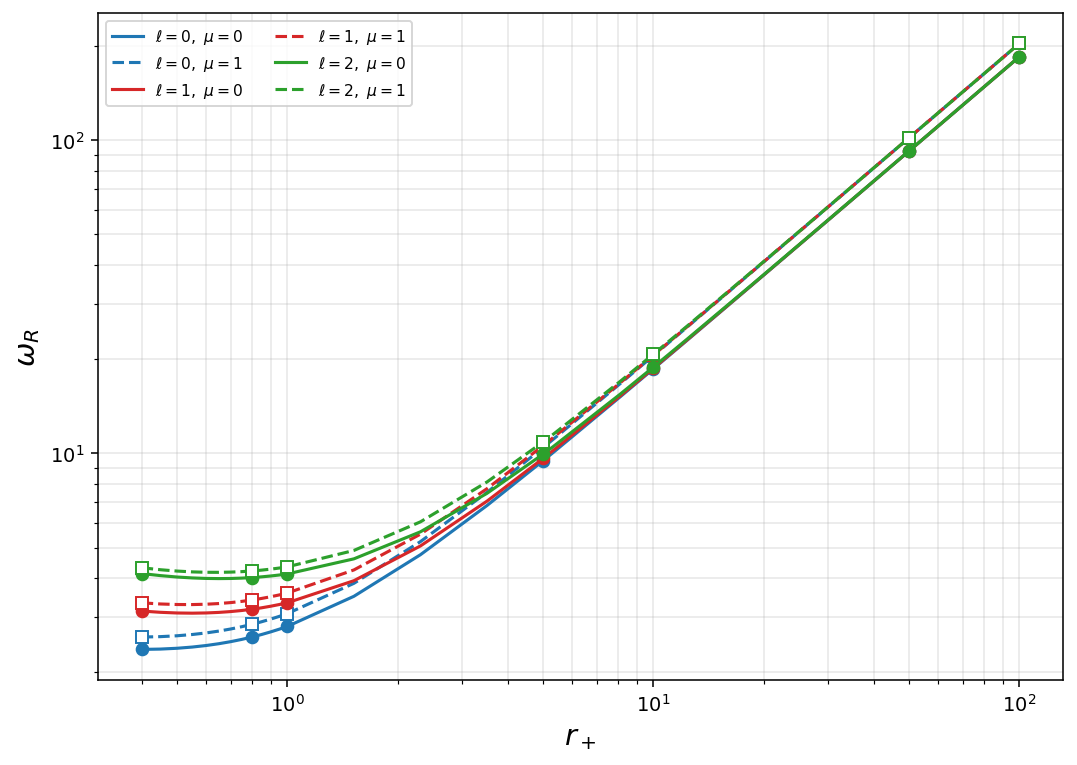
\includegraphics[width=\linewidth]{uploads/Gambar Hasil/grafik_sads_n0_wR.png}
\caption{$\omega_R$ terhadap jari-jari horizon peristiwa.}
\label{fig:sads_n0_wR}
\end{subfigure}

\caption{
Perbandingan spektrum frekuensi mode kuasinormal medan skalar pada ruang-waktu Schwarzschild Anti-de Sitter terhadap nilai jari-jari horizon peristiwa ($r_+$) untuk mode fundamental ($n=0$). Garis penuh menyatakan medan skalar tak bermassa ($\mu=0$), sedangkan garis putus-putus menyatakan medan skalar bermassa ($\mu=1$). Kurva berwarna biru, merah, dan hijau masing-masing merepresentasikan momentum sudut $\ell=0$, $\ell=1$, dan $\ell=2$.
}
\label{fig:sads_n0}

\end{figure}

Gambar~\ref{fig:sads_n0} menampilkan tren pada Tabel~\ref{tab:sads_mu0_n0} dan Tabel~\ref{tab:sads_mu1_n0} secara visual. Seluruh kurva untuk berbagai momentum sudut maupun massa medan tampak menyatu rapat pada $r_+$ besar, memvisualisasikan secara langsung memudarnya pengaruh $\ell$ dan $\mu$ yang telah dibahas sebelumnya, sedangkan perbedaan antar kurva hanya tampak jelas pada $r_+$ kecil.

\begin{figure}[H]
\centering

\begin{subfigure}[t]{0.48\textwidth}
\centering
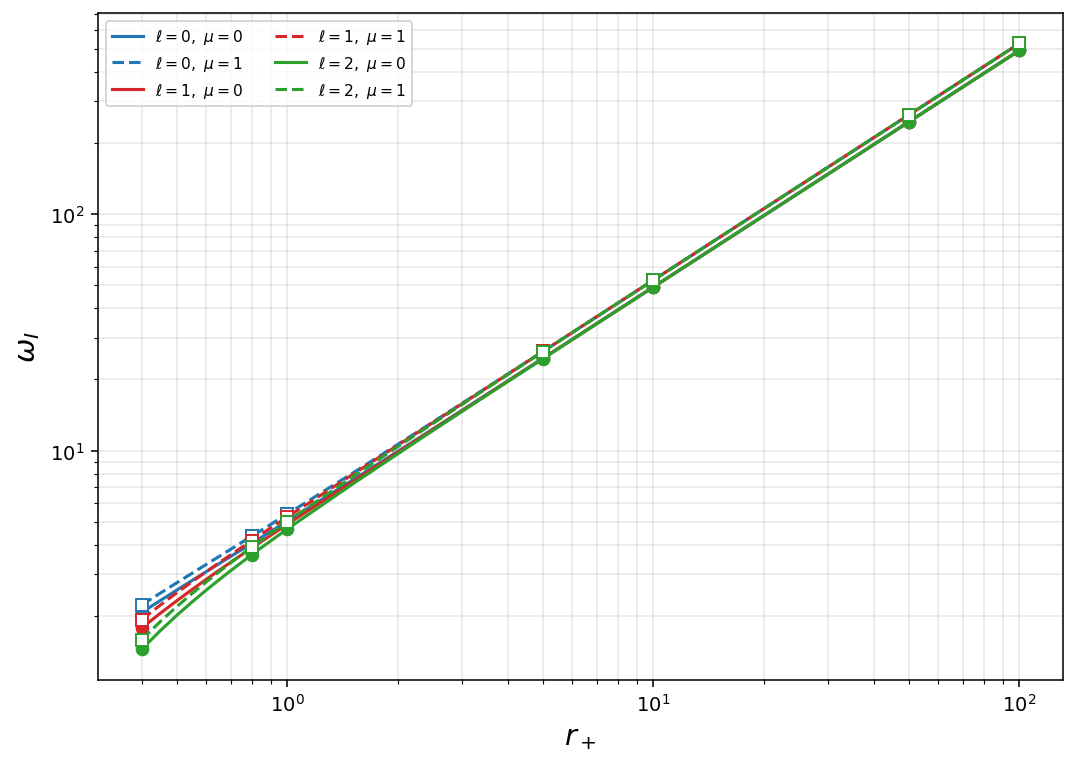
\includegraphics[width=\linewidth]{uploads/Gambar Hasil/grafik_sads_n1_wI.png}
\caption{$\omega_I$ terhadap jari-jari horizon peristiwa.}
\label{fig:sads_n1_wI}
\end{subfigure}
\hfill
\begin{subfigure}[t]{0.48\textwidth}
\centering
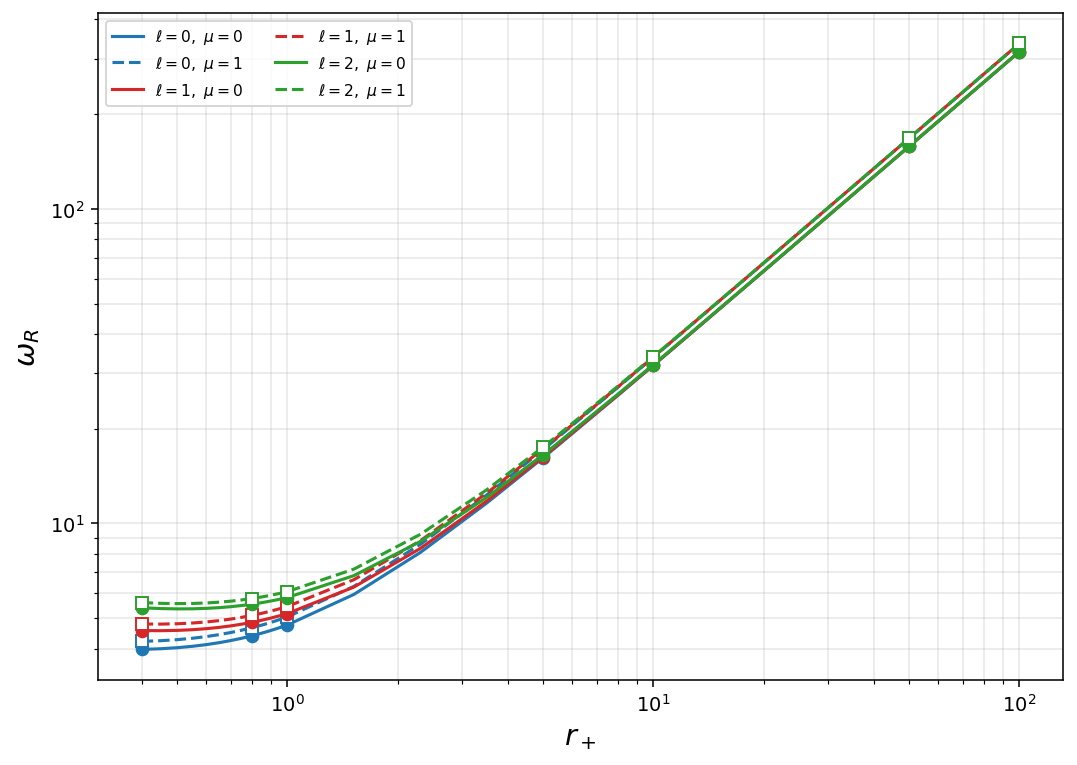
\includegraphics[width=\linewidth]{uploads/Gambar Hasil/grafik_sads_n1_wR.png}
\caption{$\omega_R$ terhadap jari-jari horizon peristiwa.}
\label{fig:sads_n1_wR}
\end{subfigure}

\caption{
Perbandingan spektrum frekuensi mode kuasinormal medan skalar pada ruang-waktu Schwarzschild Anti-de Sitter terhadap nilai jari-jari horizon peristiwa ($r_+$) untuk overtone pertama ($n=1$). Garis penuh menyatakan medan skalar tak bermassa ($\mu=0$), sedangkan garis putus-putus menyatakan medan skalar bermassa ($\mu=1$). Kurva berwarna biru, merah, dan hijau masing-masing merepresentasikan momentum sudut $\ell=0$, $\ell=1$, dan $\ell=2$.
}
\label{fig:sads_n1}

\end{figure}

Kecenderungan yang sama juga terlihat pada Gambar~\ref{fig:sads_n1} untuk overtone pertama, dengan seluruh kurva tetap menyatu pada $r_+$ besar dan hanya bercabang pada $r_+$ kecil. Bentuk kurva yang hampir identik dengan Gambar~\ref{fig:sads_n0} menegaskan bahwa kenaikan indeks overtone tidak mengubah pola ketergantungan spektrum frekuensi terhadap ukuran horizon peristiwa, melainkan hanya menggeser posisi kurva ke nilai frekuensi yang lebih tinggi.

Perbandingan antara Tabel \ref{tab:sads_mu0_n1} dan Tabel \ref{tab:sads_mu1_n1} juga menunjukkan bahwa penambahan massa medan menyebabkan terjadinya pergeseran spektrum frekuensi pada seluruh variasi jari-jari horizon peristiwa. Secara umum, bagian real frekuensi mengalami peningkatan dibandingkan kasus medan skalar tak bermassa. Sementara itu, bagian imajiner frekuensi juga meningkat sebagai akibat adanya massa medan. Hal tersebut menunjukkan bahwa massa medan skalar memberikan kontribusi terhadap karakteristik osilasi maupun laju peluruhan perturbasi pada seluruh parameter yang ditinjau.

Pengaruh momentum sudut juga menunjukkan kecenderungan yang serupa dengan hasil-hasil sebelumnya, yaitu bergantung pada ukuran horizon peristiwa. Pada $r_+$ kecil, peningkatan momentum sudut dari $\ell=0$ hingga $\ell=2$ menyebabkan perubahan yang cukup besar pada kedua komponen frekuensi; sebagai contoh, pada $r_+=0.4$, bagian real meningkat dari $4.2199$ menjadi $5.6061$, sedangkan bagian imajiner menurun dari $2.2295$ menjadi $1.5898$. Sebaliknya, pada $r_+$ besar, pengaruh momentum sudut terhadap kedua komponen frekuensi menjadi semakin kecil hingga hampir tidak teramati.

Secara keseluruhan, hasil pada Tabel \ref{tab:sads_mu0_n0} hingga Tabel \ref{tab:sads_mu1_n1} menunjukkan bahwa spektrum frekuensi mode kuasinormal pada ruang-waktu Schwarzschild Anti-de Sitter dipengaruhi oleh ukuran horizon peristiwa, massa medan skalar, dan indeks overtone secara konsisten di seluruh rentang parameter, sedangkan momentum sudut memberikan pengaruh yang signifikan terutama pada horizon peristiwa berukuran kecil. Untuk memperjelas kecenderungan tersebut, keseluruhan hasil yang didapatkan divisualisasikan dalam bentuk grafik pada Gambar~\ref{fig:sads_n0} dan Gambar~\ref{fig:sads_n1} untuk memudahkan pengamatan terhadap perubahan bagian real maupun bagian imajiner frekuensi serta perbandingan antara medan skalar tak bermassa dan bermassa.